
\documentclass[11pt]{article}\usepackage[]{graphicx}\usepackage[]{color}
%% maxwidth is the original width if it is less than linewidth
%% otherwise use linewidth (to make sure the graphics do not exceed the margin)
\makeatletter
\def\maxwidth{ %
  \ifdim\Gin@nat@width>\linewidth
    \linewidth
  \else
    \Gin@nat@width
  \fi
}
\makeatother

\definecolor{fgcolor}{rgb}{0.345, 0.345, 0.345}
\newcommand{\hlnum}[1]{\textcolor[rgb]{0.686,0.059,0.569}{#1}}%
\newcommand{\hlstr}[1]{\textcolor[rgb]{0.192,0.494,0.8}{#1}}%
\newcommand{\hlcom}[1]{\textcolor[rgb]{0.678,0.584,0.686}{\textit{#1}}}%
\newcommand{\hlopt}[1]{\textcolor[rgb]{0,0,0}{#1}}%
\newcommand{\hlstd}[1]{\textcolor[rgb]{0.345,0.345,0.345}{#1}}%
\newcommand{\hlkwa}[1]{\textcolor[rgb]{0.161,0.373,0.58}{\textbf{#1}}}%
\newcommand{\hlkwb}[1]{\textcolor[rgb]{0.69,0.353,0.396}{#1}}%
\newcommand{\hlkwc}[1]{\textcolor[rgb]{0.333,0.667,0.333}{#1}}%
\newcommand{\hlkwd}[1]{\textcolor[rgb]{0.737,0.353,0.396}{\textbf{#1}}}%

\usepackage{framed}
\makeatletter
\newenvironment{kframe}{%
 \def\at@end@of@kframe{}%
 \ifinner\ifhmode%
  \def\at@end@of@kframe{\end{minipage}}%
  \begin{minipage}{\columnwidth}%
 \fi\fi%
 \def\FrameCommand##1{\hskip\@totalleftmargin \hskip-\fboxsep
 \colorbox{shadecolor}{##1}\hskip-\fboxsep
     % There is no \\@totalrightmargin, so:
     \hskip-\linewidth \hskip-\@totalleftmargin \hskip\columnwidth}%
 \MakeFramed {\advance\hsize-\width
   \@totalleftmargin\z@ \linewidth\hsize
   \@setminipage}}%
 {\par\unskip\endMakeFramed%
 \at@end@of@kframe}
\makeatother

\definecolor{shadecolor}{rgb}{.97, .97, .97}
\definecolor{messagecolor}{rgb}{0, 0, 0}
\definecolor{warningcolor}{rgb}{1, 0, 1}
\definecolor{errorcolor}{rgb}{1, 0, 0}
\newenvironment{knitrout}{}{} % an empty environment to be redefined in TeX

\usepackage{alltt}

% Use fancy fonts
\usepackage{fontspec}
\setmainfont{Calibri}
\setsansfont{SourceSansPro-Regular}
\setmonofont{Consolas}

% pretty URLs
\usepackage{hyperref}
\hypersetup{
  colorlinks=true,
  linkcolor=black,
  citecolor=black,
  filecolor=black,
  urlcolor=blue
}
\urlstyle{sf}

% authors + affiliations
\usepackage{authblk}

% biblio
\usepackage{natbib}

% can use captions outside figure environments
\usepackage{capt-of}

% Latex special characters are rendered correctly with XeTeX
\usepackage{xltxtra}
\usepackage{xunicode}
\defaultfontfeatures{Mapping=tex-text}

% margins
\usepackage[margin=1in]{geometry}

% title
\title{Using iNaturalist to learn more about echinoderms}

\author{Fran\c{c}ois Michonneau}
\author{Gustav Paulay}
\affil{Florida Museum of Natural History, University of Florida, Gainesville,
  FL 32611-7800, USA; emails: francois.michonneau@gmail.com, paulay@flmnh.ufl.edu}

\date{}

\renewcommand\Authands{ and }

% -------------------   end of header
\IfFileExists{upquote.sty}{\usepackage{upquote}}{}
\begin{document}







\maketitle

%----------------------      paper starts here    ----------------------------%

\section*{Context}

Echinoderms are among the most conspicuous and abundant marine
invertebrates. Several species of echinoderms undergo important demographic
fluctuations, with important ecological consequences, for reasons that are not
always well understood (e.g., crown-of-thorns outbreaks, \textit{Diadema
  antillarum} die-off, starfish-wasting-syndrome, reviewed in
\citealt{Uthicke2009}). In addition, many species are targeted by unregulated
fisheries (e.g., \citealt{Purcell2014}).

Despite these factors, echinoderms have not received a lot of taxonomic
attention, and many large species remain undescribed and/or poorly
known. Regularly, field guides illustrate undescribed species, and divers
commonly photograph new or poorly known species. 

With recent technological advances, it has become increasingly easier to
document species encountered in nature. For instance, smartphones can, with the
single touch of the screen, take a picture while associating the exact
geographical location and time of the observation. Digital cameras have made
underwater photography much more accessible, and many divers now document the
species they encounter by sharing their pictures on social media websites.

Our knowledge of echinoderms could therefore be improved by aggregating user
observations of these organisms, while, at the same time, educating the public
about the diversity and natural history of these fascinating organisms.

\section*{What is iNaturalist?}

iNaturalist (\href{http://inaturalist.org}{http://inaturalist.org}) is a website
that allows users to submit observations about any species (on land or
underwater), along with images, GPS coordinates and ancillary information about
the habitat or natural history (Figure~\ref{fig:example-observation}). Once
submitted, the observations can be further identified by the community and
validated by "curators" (users with recognized knowledge of a given taxonomic
group whose opinion can be trusted). This mechanism allows users to hone their
identification skills, learn about the organisms, and communicate with each
other. Observations, in turn, provide a wealth of information about
distribution, variation, abundance, and other aspects of natural history.

\begin{center}
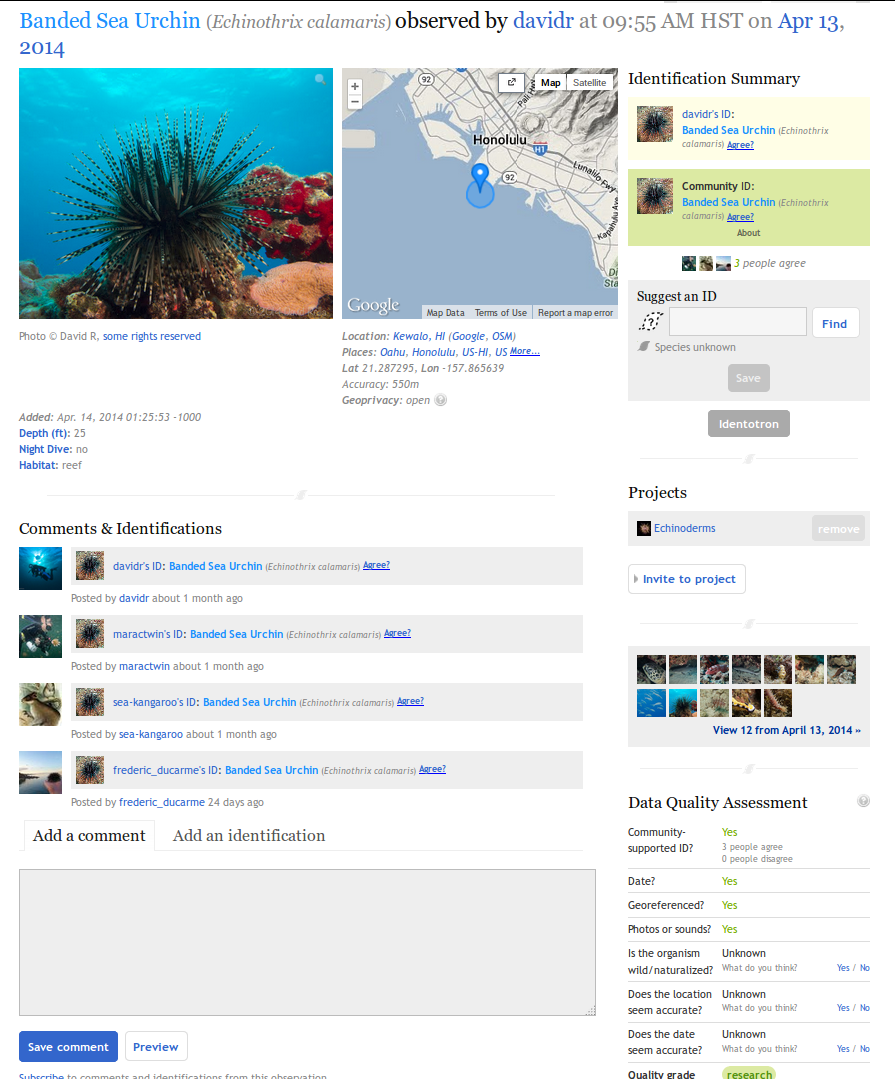
\includegraphics[width=.5\columnwidth]{images/inat-screenshot}
\captionof{figure}{Example of an user-submitted observation}
\label{fig:example-observation}
\end{center}

\section*{The Echinoderm project on iNaturalist}

We started a project on Echinoderms
(\href{http://inaturalist.org/projects/echinoderms}{http://inaturalist.org/projects/echinoderms})
to gather observations worldwide, and across taxa. Our goal is to improve our
knowledge of species distributions, variation, and biology, and to educate the
public about the diversity of echinoderms. This platform provides a great
outreach tool facilitating communication between scientists and
naturalists. Because iNaturalist is easy to use and has applications for mobile
devices, it can also be used during organized citizen science initiatives such
as Bioblitz, or class field trips.

Beyond outreach, iNaturalist can be a useful tool for scientists. Echinoderms
are among the few mobile invertebrate regularly recorded in coral reef ecosystem
monitoring. By submitting species observations on iNaturalist, data will be
archived, accessible, and shareable with the community. Additionally, it is also
an opportunity to obtain accurate identification for the species encountered
with the help of the community.

The aggregated data is made openly available and can be used by scientists to
study demographic and spatial patterns, or even to infer distributions using
ecological niche modeling. For instance, recent taxonomic research on sea
cucumbers has shown that species can be told apart based on their color patterns
(e.g., \citealt{Kim2013,Kerr2013}). However, taxonomic confusion through the
years has hindered our knowledge of species distributions, as the incorrect
species names have extensively been used in the literature. Having photographic
evidence associated with geographical data will allow to validate geographical
distributions once taxonomic research has clarified species limits. Furthermore,
iNaturalist could be very useful to track through space and time changes in
species abundance during a crown-of-thorns outbreak for instance.

\section*{Present and future observations}

Since the beginning of the project in March 2014, over a hundred users have
already contributed 850+ echinoderm observations worldwide. Currently, large and
abundant species from the intertidal of the Western United States dominate,
reflecting the development of iNaturalist in California
(Figure~\ref{fig:all-observations}). However, underwater sightings from the
Caribbean and the Indo-West Pacific also represent a large proportion of the
observations and indicate the potential of iNaturalist to document marine
invertebrate biodiversity.

We aim at expanding both taxonomic and geographic coverage. Many species of
echinoderms can be found associated with coral reefs, and for most, their
geographical distribution is poorly known. Reef scientists can improve our
knowledge of their distribution by reporting the species they see in the
field. Additionally, we are in the process of advertising the project to the
SCUBA diving community and through citizen science initiatives to increase
participation.

We welcome everyone to submit their echinoderm observations, or help curating
the records submitted to the project. Don't hesitate to join us!

\begin{center}
\begin{knitrout}
\definecolor{shadecolor}{rgb}{0.969, 0.969, 0.969}\color{fgcolor}
\includegraphics[width=\columnwidth]{figures/latex-all-observations} 

\end{knitrout}
\captionof{figure}{Global distribution of observations recorded by iNaturalist
  users as of May 29th, 2014 per class}
\label{fig:all-observations}
\end{center}

\section*{Methods}

{\small This article is open-source (CC-BY), fully reproducible and available on
  github
  (\href{https://github.com/fmichonneau/inat-paper/}{http://github.com/fmichonneau/inat-paper}). It
  was made possible using R \citep{Rproject} complemented with the packages
  ggplot2 \citep{Wickham2009}, knitr \citep{Xie2014}, taxize
  \citep{Chamberlain2013,Chamberlain2014}, and wesanderson \citep{Ram2014}.  }

\bibliographystyle{coral-reefs}

\bibliography{iNaturalist-nourl}

\end{document}
